\documentclass[12pt,a4paper]{article}
\usepackage{url}
\usepackage[backend=bibtex]{biblatex}
\usepackage{caption}
\usepackage[utf8]{inputenc}
\usepackage{enumerate}
\usepackage{tabularx}
\usepackage{graphicx}
\usepackage{float}
\usepackage{amssymb,amsmath,wasysym}


\begin{document}

\title{Computational Intelligence, SS2017, Assigment 2}

\author{%
\name{Lucas Reeh}
\email{lreeh@student.tugraz.at}
}
\date{\today}

\begin{titlepage}
   \begin{center}
     \begin{huge}
		   %% Update assignment number here
           \textbf{Assignment 2}
     \end{huge}
   \end{center}

   \begin{center}
     \begin{large}
           Computational Intelligence, SS2017
     \end{large}
   \end{center}

   \begin{center}
 \begin{tabularx}{\textwidth}{|>{\hsize=.33\hsize}X|>{\hsize=.33\hsize}X|>{\hsize=.33\hsize}X|} 

           \hline
           \multicolumn{3}{|c|}{\textbf{Team Members}} \\
           \hline
           Last name & First name & Matriculation Number \\
           \hline
           Reeh & Lucas & 00630128 \\
           \hline

     \end{tabularx}
   \end{center}
\end{titlepage}

\tableofcontents
\listoffigures

\newpage

\section{Regression with Neural Networks}

\subsubsection{Simple Regression with Neural Networks}

\begin{enumerate}[a)]
  
%%%%%%%%%%%%%%%%%%%%%%%%%% 1.1 a)
  
  \item \textbf{Learned function}
  
\begin{figure}[H]
	\centering
  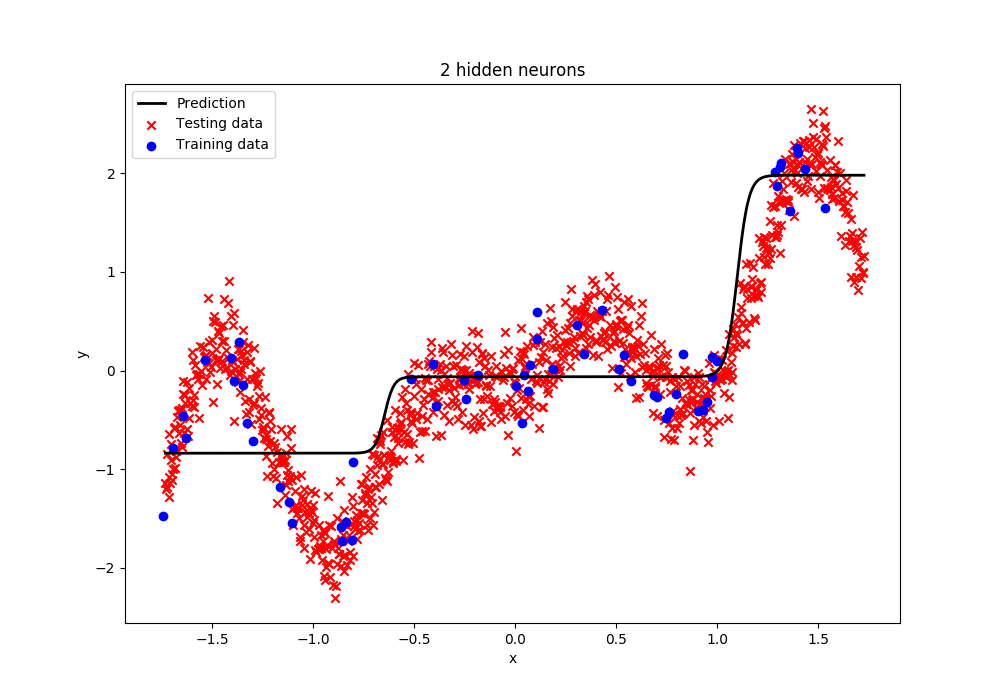
\includegraphics[width=\textwidth]{figures/1_1_a_hn_2.png}
	\caption{NN Learned function $h_n=2$}
	\label{1_1_a_hn_2}
\end{figure}

\begin{figure}[H]
	\centering
  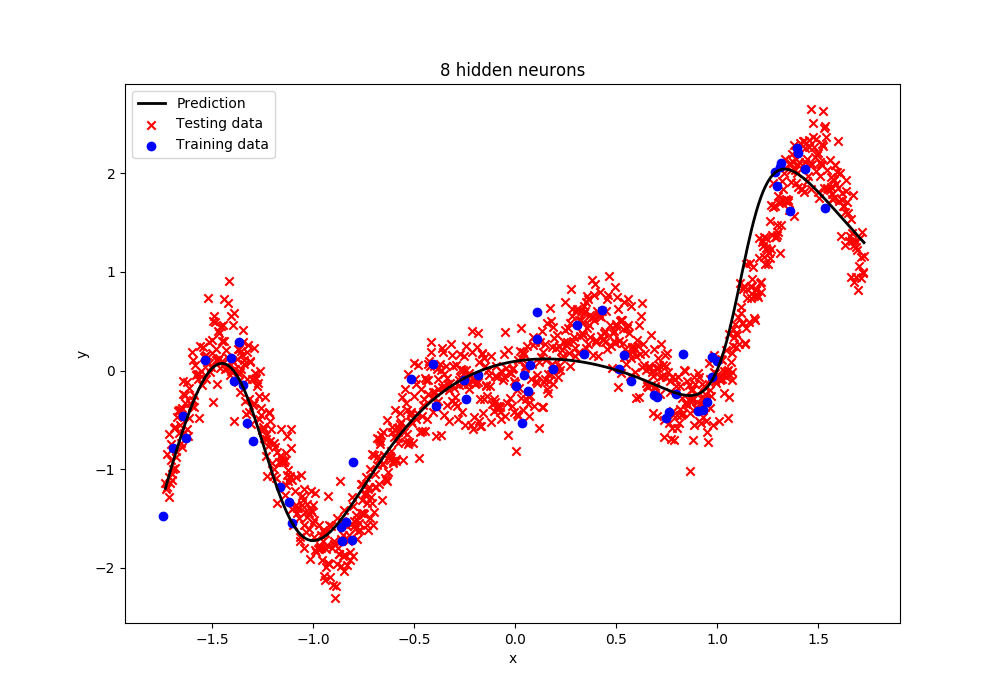
\includegraphics[width=\textwidth]{figures/1_1_a_hn_8.png}
	\caption{NN Learned function $h_n=8$}
	\label{1_1_a_hn_8}
\end{figure}

\begin{figure}[H]
	\centering
  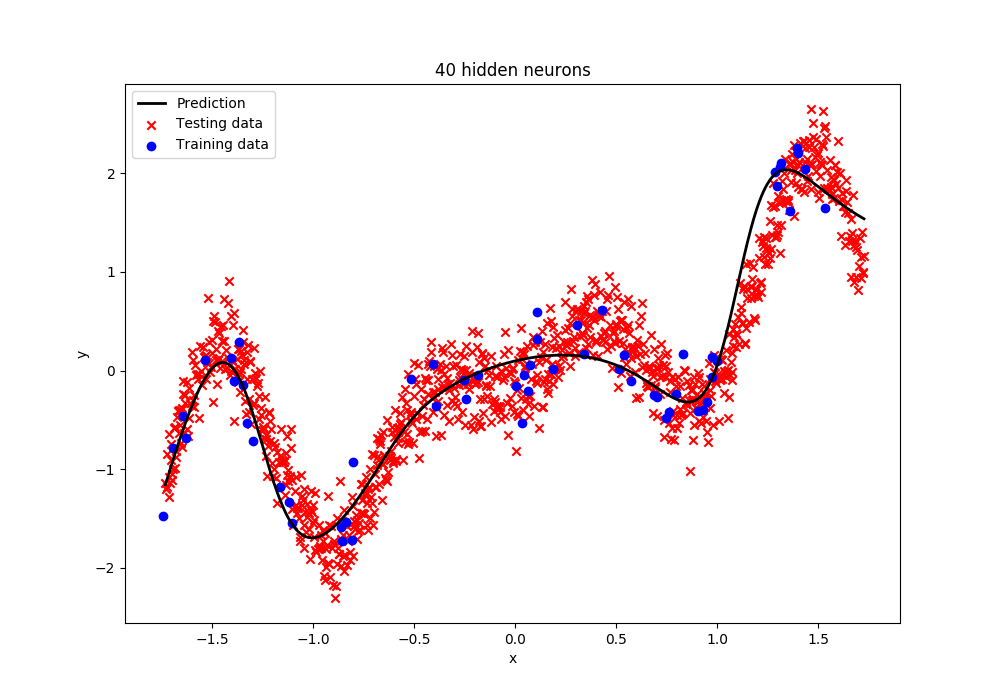
\includegraphics[width=\textwidth]{figures/1_1_a_hn_40.png}
	\caption{NN Learned function $h_n=40$}
	\label{1_1_a_hn_40}
\end{figure}
  
\textbf{Discussion: } $2$ hidden layer are cleary an underfitting
parametrization (missing a lot of data points), $h_n = 8$ seems to miss data
points where $ x = 0.0$, $40$ hidden layer tend to overfit a little (see slope
around $x = 1.5$ is going up again). As shown in Figure \ref{1_1_a_hn_100} $100$
hidden layers seem to recognize the concarve slope around $x = 0.0$ but is also
overfitting at $x > 1.2$.

\begin{figure}[H]
	\centering
  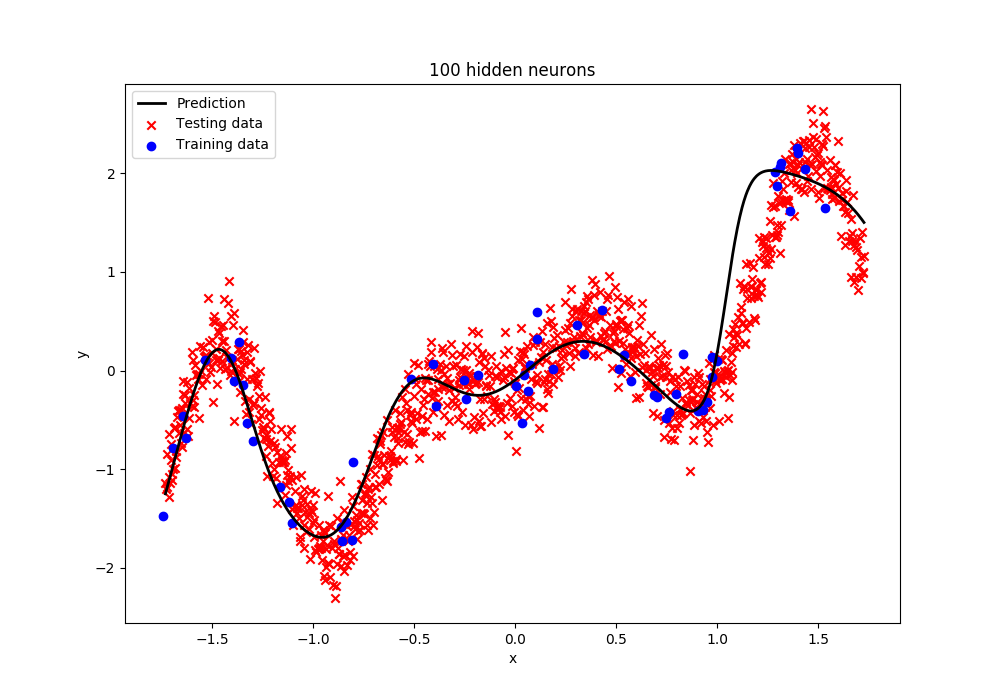
\includegraphics[width=\textwidth]{figures/1_1_a_hn_100.png}
	\caption{NN Learned function $h_n=100$}
	\label{1_1_a_hn_100}
\end{figure}

%%%%%%%%%%%%%%%%%%%%%%%%%% 1.1 b)

  \item \textbf{Variability of the performance of deep neural networks}

Result for \texttt{seed\_state} = $1..9$:


\texttt{Training MSE \\
- min = 0.040917789313120616 \\
- max = 0.05225074774663281 \\
- mean = 0.0449607719274836 \\
- std = 0.003249135660634265 \\
\\
Test MSE \\
- min = 0.09765403812014457 \\
- max = 0.23390967685837927 \\
- mean = 0.16488353377213483 \\
- std = 0.04044808429648212\\
}

\begin{itemize}
  \item The min MSE is not the same on test and training set.
  \item On small data various sets different seeds can lead to
  over-/underfitting as well es high variance.
\end{itemize}

  \item \textbf{Varying the number of hidden neurons}
  
\begin{figure}[H]
	\centering
  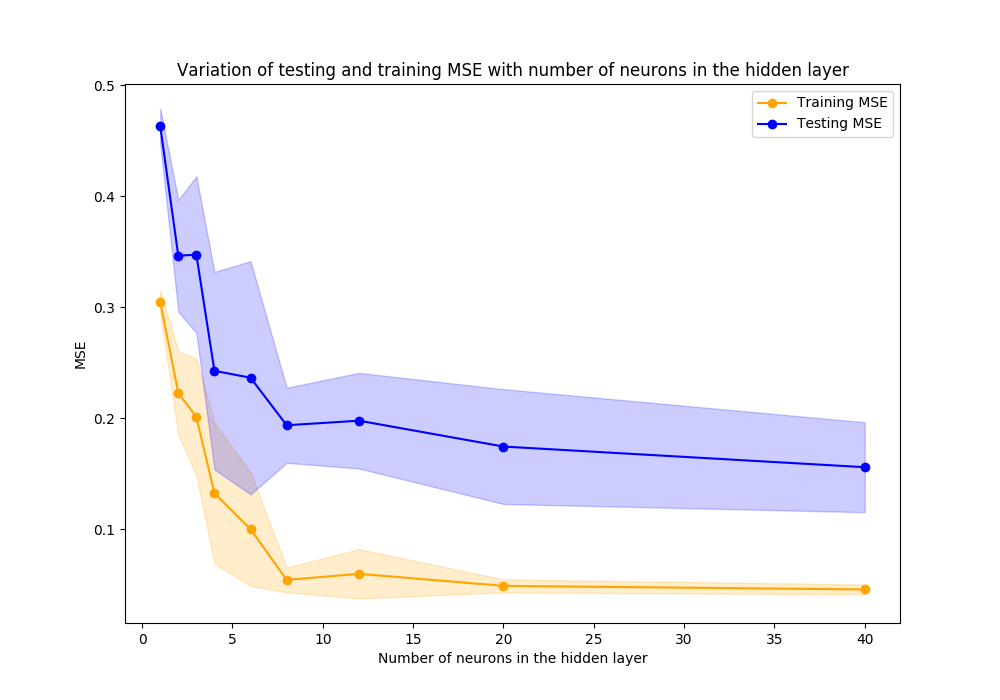
\includegraphics[width=\textwidth]{figures/1_1_c.png}
	\caption{Varying the number of hidden neurons}
	\label{1_1_c}
\end{figure}

\begin{itemize}
  \item Best $h_n$ would be $40$ on the Testing Set and $20$ (already) on the
  Training Set (recommend ``Early Stopping'').
  \item Starting with a little underfitting but getting less with growing $h_n$
\end{itemize}

\end{enumerate}


\end{document}